%VÝKON NA PROUDU
\begin{tabulka}[htbp]
\centering
\begin{tabular}{c|c}
proud výbojovou trubicí (\si{\mA}) & relativní intenzita \\ \hline
6,50 & 80 \\
6,00 & 78 \\
5,50 & 74 \\
5,00 & 70 \\
4,50 & 66 \\
\end{tabular}
\caption{Závislost relativní intenzity na proudu výbojovou trubicí}
\label{t:proud}
\end{tabulka}


\begin{graph}[htbp]
\centering
% GNUPLOT: LaTeX picture with Postscript
\begingroup
  \makeatletter
  \providecommand\color[2][]{%
    \GenericError{(gnuplot) \space\space\space\@spaces}{%
      Package color not loaded in conjunction with
      terminal option `colourtext'%
    }{See the gnuplot documentation for explanation.%
    }{Either use 'blacktext' in gnuplot or load the package
      color.sty in LaTeX.}%
    \renewcommand\color[2][]{}%
  }%
  \providecommand\includegraphics[2][]{%
    \GenericError{(gnuplot) \space\space\space\@spaces}{%
      Package graphicx or graphics not loaded%
    }{See the gnuplot documentation for explanation.%
    }{The gnuplot epslatex terminal needs graphicx.sty or graphics.sty.}%
    \renewcommand\includegraphics[2][]{}%
  }%
  \providecommand\rotatebox[2]{#2}%
  \@ifundefined{ifGPcolor}{%
    \newif\ifGPcolor
    \GPcolorfalse
  }{}%
  \@ifundefined{ifGPblacktext}{%
    \newif\ifGPblacktext
    \GPblacktexttrue
  }{}%
  % define a \g@addto@macro without @ in the name:
  \let\gplgaddtomacro\g@addto@macro
  % define empty templates for all commands taking text:
  \gdef\gplbacktext{}%
  \gdef\gplfronttext{}%
  \makeatother
  \ifGPblacktext
    % no textcolor at all
    \def\colorrgb#1{}%
    \def\colorgray#1{}%
  \else
    % gray or color?
    \ifGPcolor
      \def\colorrgb#1{\color[rgb]{#1}}%
      \def\colorgray#1{\color[gray]{#1}}%
      \expandafter\def\csname LTw\endcsname{\color{white}}%
      \expandafter\def\csname LTb\endcsname{\color{black}}%
      \expandafter\def\csname LTa\endcsname{\color{black}}%
      \expandafter\def\csname LT0\endcsname{\color[rgb]{1,0,0}}%
      \expandafter\def\csname LT1\endcsname{\color[rgb]{0,1,0}}%
      \expandafter\def\csname LT2\endcsname{\color[rgb]{0,0,1}}%
      \expandafter\def\csname LT3\endcsname{\color[rgb]{1,0,1}}%
      \expandafter\def\csname LT4\endcsname{\color[rgb]{0,1,1}}%
      \expandafter\def\csname LT5\endcsname{\color[rgb]{1,1,0}}%
      \expandafter\def\csname LT6\endcsname{\color[rgb]{0,0,0}}%
      \expandafter\def\csname LT7\endcsname{\color[rgb]{1,0.3,0}}%
      \expandafter\def\csname LT8\endcsname{\color[rgb]{0.5,0.5,0.5}}%
    \else
      % gray
      \def\colorrgb#1{\color{black}}%
      \def\colorgray#1{\color[gray]{#1}}%
      \expandafter\def\csname LTw\endcsname{\color{white}}%
      \expandafter\def\csname LTb\endcsname{\color{black}}%
      \expandafter\def\csname LTa\endcsname{\color{black}}%
      \expandafter\def\csname LT0\endcsname{\color{black}}%
      \expandafter\def\csname LT1\endcsname{\color{black}}%
      \expandafter\def\csname LT2\endcsname{\color{black}}%
      \expandafter\def\csname LT3\endcsname{\color{black}}%
      \expandafter\def\csname LT4\endcsname{\color{black}}%
      \expandafter\def\csname LT5\endcsname{\color{black}}%
      \expandafter\def\csname LT6\endcsname{\color{black}}%
      \expandafter\def\csname LT7\endcsname{\color{black}}%
      \expandafter\def\csname LT8\endcsname{\color{black}}%
    \fi
  \fi
  \setlength{\unitlength}{0.0500bp}%
  \begin{picture}(7936.00,3968.00)%
    \gplgaddtomacro\gplbacktext{%
      \csname LTb\endcsname%
      \put(814,704){\makebox(0,0)[r]{\strut{} 65}}%
      \csname LTb\endcsname%
      \put(814,1454){\makebox(0,0)[r]{\strut{} 70}}%
      \csname LTb\endcsname%
      \put(814,2204){\makebox(0,0)[r]{\strut{} 75}}%
      \csname LTb\endcsname%
      \put(814,2953){\makebox(0,0)[r]{\strut{} 80}}%
      \csname LTb\endcsname%
      \put(814,3703){\makebox(0,0)[r]{\strut{} 85}}%
      \csname LTb\endcsname%
      \put(946,484){\makebox(0,0){\strut{} 4}}%
      \csname LTb\endcsname%
      \put(2045,484){\makebox(0,0){\strut{} 4.5}}%
      \csname LTb\endcsname%
      \put(3144,484){\makebox(0,0){\strut{} 5}}%
      \csname LTb\endcsname%
      \put(4243,484){\makebox(0,0){\strut{} 5.5}}%
      \csname LTb\endcsname%
      \put(5341,484){\makebox(0,0){\strut{} 6}}%
      \csname LTb\endcsname%
      \put(6440,484){\makebox(0,0){\strut{} 6.5}}%
      \csname LTb\endcsname%
      \put(7539,484){\makebox(0,0){\strut{} 7}}%
      \put(176,2203){\rotatebox{-270}{\makebox(0,0){\strut{}relativní intenzita}}}%
      \put(4242,154){\makebox(0,0){\strut{}proud výbojovou trubicí (\si{\mA})}}%
    }%
    \gplgaddtomacro\gplfronttext{%
    }%
    \gplbacktext
    \put(0,0){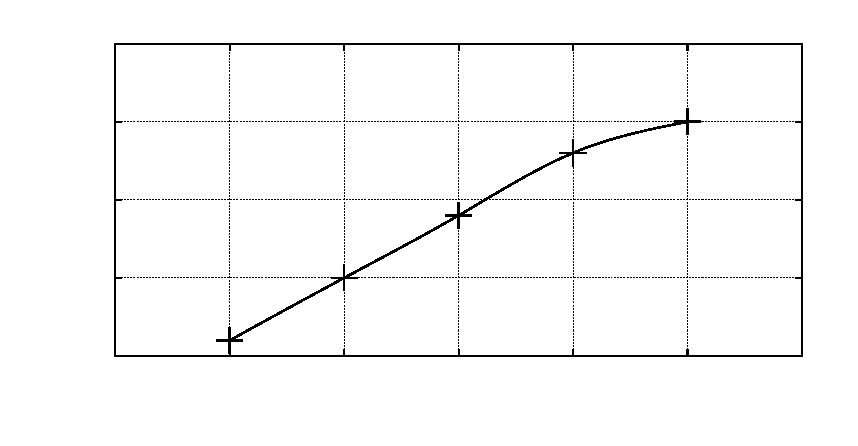
\includegraphics{proud}}%
    \gplfronttext
  \end{picture}%
\endgroup

\caption{Závislost relativní intenzity na proudu výbojovou trubicí}
\label{g:proud}
\end{graph}


%PROFIL SVAZKU
\begin{tabulka}[htbp]
\centering
\begin{tabular}{cc||cc||cc}
$x$ (\si{\mm}) & $I$ & $x$ (\si{\mm}) & $I$ & $x$ (\si{\mm}) & $I$ \\ \hline
15,45 & 6 & 15,90 & 60 & 16,35 & 78 \\ 
15,50 & 14 & 15,95 & 64 & 16,40 & 72 \\ 
15,55 & 14 & 16,00 & 70 & 16,45 & 60 \\ 
15,60 & 18 & 16,05 & 76 & 16,50 & 50 \\ 
15,65 & 24 & 16,10 & 80 & 16,55 & 38 \\ 
15,70 & 34 & 16,15 & 84 & 16,60 & 28 \\ 
15,75 & 40 & 16,20 & 82 & 16,65 & 14 \\ 
15,80 & 44 & 16,25 & 82 & 16,70 & 8 \\ 
15,85 & 52 & 16,30 & 82 & 16,75 & 4 \\ 
\end{tabular}
\caption{Měření profilu svazku, $I$ je intenzita v relativních jednotkách}
\label{t:profil}
\end{tabulka}


\begin{graph}[htbp] 
\centering
% GNUPLOT: LaTeX picture with Postscript
\begingroup
  \makeatletter
  \providecommand\color[2][]{%
    \GenericError{(gnuplot) \space\space\space\@spaces}{%
      Package color not loaded in conjunction with
      terminal option `colourtext'%
    }{See the gnuplot documentation for explanation.%
    }{Either use 'blacktext' in gnuplot or load the package
      color.sty in LaTeX.}%
    \renewcommand\color[2][]{}%
  }%
  \providecommand\includegraphics[2][]{%
    \GenericError{(gnuplot) \space\space\space\@spaces}{%
      Package graphicx or graphics not loaded%
    }{See the gnuplot documentation for explanation.%
    }{The gnuplot epslatex terminal needs graphicx.sty or graphics.sty.}%
    \renewcommand\includegraphics[2][]{}%
  }%
  \providecommand\rotatebox[2]{#2}%
  \@ifundefined{ifGPcolor}{%
    \newif\ifGPcolor
    \GPcolorfalse
  }{}%
  \@ifundefined{ifGPblacktext}{%
    \newif\ifGPblacktext
    \GPblacktexttrue
  }{}%
  % define a \g@addto@macro without @ in the name:
  \let\gplgaddtomacro\g@addto@macro
  % define empty templates for all commands taking text:
  \gdef\gplbacktext{}%
  \gdef\gplfronttext{}%
  \makeatother
  \ifGPblacktext
    % no textcolor at all
    \def\colorrgb#1{}%
    \def\colorgray#1{}%
  \else
    % gray or color?
    \ifGPcolor
      \def\colorrgb#1{\color[rgb]{#1}}%
      \def\colorgray#1{\color[gray]{#1}}%
      \expandafter\def\csname LTw\endcsname{\color{white}}%
      \expandafter\def\csname LTb\endcsname{\color{black}}%
      \expandafter\def\csname LTa\endcsname{\color{black}}%
      \expandafter\def\csname LT0\endcsname{\color[rgb]{1,0,0}}%
      \expandafter\def\csname LT1\endcsname{\color[rgb]{0,1,0}}%
      \expandafter\def\csname LT2\endcsname{\color[rgb]{0,0,1}}%
      \expandafter\def\csname LT3\endcsname{\color[rgb]{1,0,1}}%
      \expandafter\def\csname LT4\endcsname{\color[rgb]{0,1,1}}%
      \expandafter\def\csname LT5\endcsname{\color[rgb]{1,1,0}}%
      \expandafter\def\csname LT6\endcsname{\color[rgb]{0,0,0}}%
      \expandafter\def\csname LT7\endcsname{\color[rgb]{1,0.3,0}}%
      \expandafter\def\csname LT8\endcsname{\color[rgb]{0.5,0.5,0.5}}%
    \else
      % gray
      \def\colorrgb#1{\color{black}}%
      \def\colorgray#1{\color[gray]{#1}}%
      \expandafter\def\csname LTw\endcsname{\color{white}}%
      \expandafter\def\csname LTb\endcsname{\color{black}}%
      \expandafter\def\csname LTa\endcsname{\color{black}}%
      \expandafter\def\csname LT0\endcsname{\color{black}}%
      \expandafter\def\csname LT1\endcsname{\color{black}}%
      \expandafter\def\csname LT2\endcsname{\color{black}}%
      \expandafter\def\csname LT3\endcsname{\color{black}}%
      \expandafter\def\csname LT4\endcsname{\color{black}}%
      \expandafter\def\csname LT5\endcsname{\color{black}}%
      \expandafter\def\csname LT6\endcsname{\color{black}}%
      \expandafter\def\csname LT7\endcsname{\color{black}}%
      \expandafter\def\csname LT8\endcsname{\color{black}}%
    \fi
  \fi
  \setlength{\unitlength}{0.0500bp}%
  \begin{picture}(10204.00,5668.00)%
    \gplgaddtomacro\gplbacktext{%
      \csname LTb\endcsname%
      \put(814,704){\makebox(0,0)[r]{\strut{} 0}}%
      \csname LTb\endcsname%
      \put(814,1226){\makebox(0,0)[r]{\strut{} 10}}%
      \csname LTb\endcsname%
      \put(814,1748){\makebox(0,0)[r]{\strut{} 20}}%
      \csname LTb\endcsname%
      \put(814,2270){\makebox(0,0)[r]{\strut{} 30}}%
      \csname LTb\endcsname%
      \put(814,2792){\makebox(0,0)[r]{\strut{} 40}}%
      \csname LTb\endcsname%
      \put(814,3315){\makebox(0,0)[r]{\strut{} 50}}%
      \csname LTb\endcsname%
      \put(814,3837){\makebox(0,0)[r]{\strut{} 60}}%
      \csname LTb\endcsname%
      \put(814,4359){\makebox(0,0)[r]{\strut{} 70}}%
      \csname LTb\endcsname%
      \put(814,4881){\makebox(0,0)[r]{\strut{} 80}}%
      \csname LTb\endcsname%
      \put(814,5403){\makebox(0,0)[r]{\strut{} 90}}%
      \csname LTb\endcsname%
      \put(946,484){\makebox(0,0){\strut{} 15.4}}%
      \csname LTb\endcsname%
      \put(2212,484){\makebox(0,0){\strut{} 15.6}}%
      \csname LTb\endcsname%
      \put(3478,484){\makebox(0,0){\strut{} 15.8}}%
      \csname LTb\endcsname%
      \put(4744,484){\makebox(0,0){\strut{} 16}}%
      \csname LTb\endcsname%
      \put(6009,484){\makebox(0,0){\strut{} 16.2}}%
      \csname LTb\endcsname%
      \put(7275,484){\makebox(0,0){\strut{} 16.4}}%
      \csname LTb\endcsname%
      \put(8541,484){\makebox(0,0){\strut{} 16.6}}%
      \csname LTb\endcsname%
      \put(9807,484){\makebox(0,0){\strut{} 16.8}}%
      \put(176,3053){\rotatebox{-270}{\makebox(0,0){\strut{}$I$}}}%
      \put(5376,154){\makebox(0,0){\strut{}$x$ (\si{\mm})}}%
    }%
    \gplgaddtomacro\gplfronttext{%
      \csname LTb\endcsname%
      \put(8820,5230){\makebox(0,0)[r]{\strut{}naměřené hodnoty}}%
      \csname LTb\endcsname%
      \put(8820,5010){\makebox(0,0)[r]{\strut{}fit Gaussovou funkcí}}%
    }%
    \gplbacktext
    \put(0,0){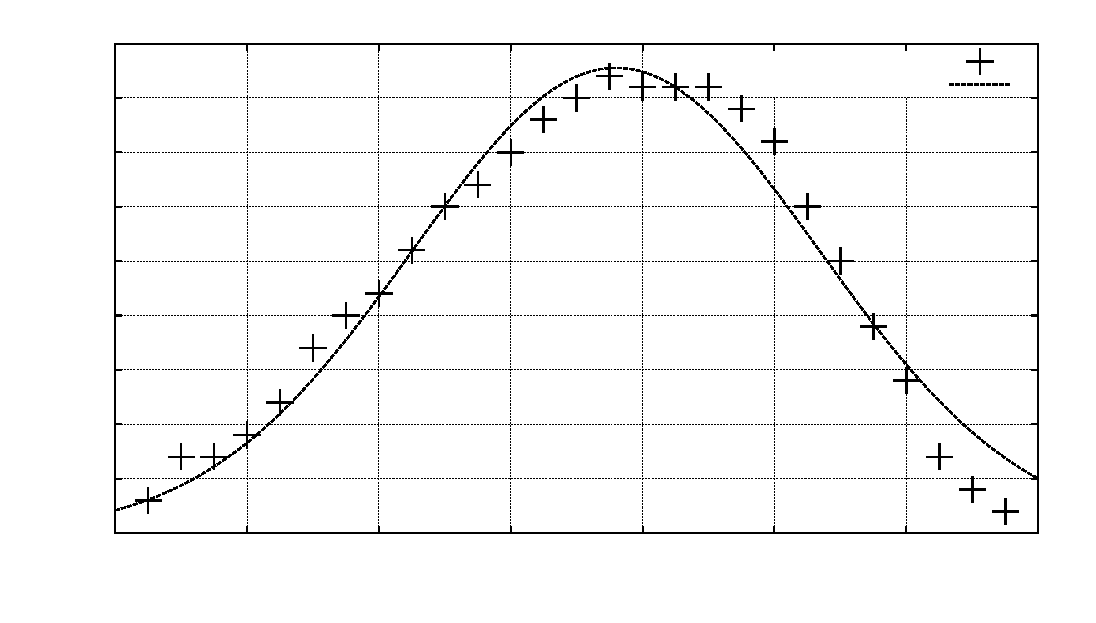
\includegraphics{profil}}%
    \gplfronttext
  \end{picture}%
\endgroup

\caption{Měření profilu svazku, $I$ je intenzita v relativních jednotkách}
\label{g:profil}
\end{graph}


%DIVERGENCE
\begin{tabulka}[htbp]
\centering
\begin{tabular}{c|c|c}
$s$ (\si{\cm}) & beam width clip (\si{\micro\metre}) & gaussian diameter (\si{\micro\metre}) \\
\hline
\num{8(1)} & 1040 & 1080 \\
\num{132(3)} & 2680 & 2830 \\
\num{243(5)} & --- & 4000 
\end{tabular}
\caption{Průměr svazku v různých vzdálenostech od výstupu laseru}
\label{t:div}
\end{tabulka}


\begin{graph}[htbp] 
\centering
% GNUPLOT: LaTeX picture with Postscript
\begingroup
  \makeatletter
  \providecommand\color[2][]{%
    \GenericError{(gnuplot) \space\space\space\@spaces}{%
      Package color not loaded in conjunction with
      terminal option `colourtext'%
    }{See the gnuplot documentation for explanation.%
    }{Either use 'blacktext' in gnuplot or load the package
      color.sty in LaTeX.}%
    \renewcommand\color[2][]{}%
  }%
  \providecommand\includegraphics[2][]{%
    \GenericError{(gnuplot) \space\space\space\@spaces}{%
      Package graphicx or graphics not loaded%
    }{See the gnuplot documentation for explanation.%
    }{The gnuplot epslatex terminal needs graphicx.sty or graphics.sty.}%
    \renewcommand\includegraphics[2][]{}%
  }%
  \providecommand\rotatebox[2]{#2}%
  \@ifundefined{ifGPcolor}{%
    \newif\ifGPcolor
    \GPcolorfalse
  }{}%
  \@ifundefined{ifGPblacktext}{%
    \newif\ifGPblacktext
    \GPblacktexttrue
  }{}%
  % define a \g@addto@macro without @ in the name:
  \let\gplgaddtomacro\g@addto@macro
  % define empty templates for all commands taking text:
  \gdef\gplbacktext{}%
  \gdef\gplfronttext{}%
  \makeatother
  \ifGPblacktext
    % no textcolor at all
    \def\colorrgb#1{}%
    \def\colorgray#1{}%
  \else
    % gray or color?
    \ifGPcolor
      \def\colorrgb#1{\color[rgb]{#1}}%
      \def\colorgray#1{\color[gray]{#1}}%
      \expandafter\def\csname LTw\endcsname{\color{white}}%
      \expandafter\def\csname LTb\endcsname{\color{black}}%
      \expandafter\def\csname LTa\endcsname{\color{black}}%
      \expandafter\def\csname LT0\endcsname{\color[rgb]{1,0,0}}%
      \expandafter\def\csname LT1\endcsname{\color[rgb]{0,1,0}}%
      \expandafter\def\csname LT2\endcsname{\color[rgb]{0,0,1}}%
      \expandafter\def\csname LT3\endcsname{\color[rgb]{1,0,1}}%
      \expandafter\def\csname LT4\endcsname{\color[rgb]{0,1,1}}%
      \expandafter\def\csname LT5\endcsname{\color[rgb]{1,1,0}}%
      \expandafter\def\csname LT6\endcsname{\color[rgb]{0,0,0}}%
      \expandafter\def\csname LT7\endcsname{\color[rgb]{1,0.3,0}}%
      \expandafter\def\csname LT8\endcsname{\color[rgb]{0.5,0.5,0.5}}%
    \else
      % gray
      \def\colorrgb#1{\color{black}}%
      \def\colorgray#1{\color[gray]{#1}}%
      \expandafter\def\csname LTw\endcsname{\color{white}}%
      \expandafter\def\csname LTb\endcsname{\color{black}}%
      \expandafter\def\csname LTa\endcsname{\color{black}}%
      \expandafter\def\csname LT0\endcsname{\color{black}}%
      \expandafter\def\csname LT1\endcsname{\color{black}}%
      \expandafter\def\csname LT2\endcsname{\color{black}}%
      \expandafter\def\csname LT3\endcsname{\color{black}}%
      \expandafter\def\csname LT4\endcsname{\color{black}}%
      \expandafter\def\csname LT5\endcsname{\color{black}}%
      \expandafter\def\csname LT6\endcsname{\color{black}}%
      \expandafter\def\csname LT7\endcsname{\color{black}}%
      \expandafter\def\csname LT8\endcsname{\color{black}}%
    \fi
  \fi
  \setlength{\unitlength}{0.0500bp}%
  \begin{picture}(7936.00,3968.00)%
    \gplgaddtomacro\gplbacktext{%
      \csname LTb\endcsname%
      \put(1078,704){\makebox(0,0)[r]{\strut{} 0}}%
      \csname LTb\endcsname%
      \put(1078,1370){\makebox(0,0)[r]{\strut{} 1000}}%
      \csname LTb\endcsname%
      \put(1078,2037){\makebox(0,0)[r]{\strut{} 2000}}%
      \csname LTb\endcsname%
      \put(1078,2703){\makebox(0,0)[r]{\strut{} 3000}}%
      \csname LTb\endcsname%
      \put(1078,3370){\makebox(0,0)[r]{\strut{} 4000}}%
      \csname LTb\endcsname%
      \put(1210,484){\makebox(0,0){\strut{} 0}}%
      \csname LTb\endcsname%
      \put(2476,484){\makebox(0,0){\strut{} 50}}%
      \csname LTb\endcsname%
      \put(3742,484){\makebox(0,0){\strut{} 100}}%
      \csname LTb\endcsname%
      \put(5007,484){\makebox(0,0){\strut{} 150}}%
      \csname LTb\endcsname%
      \put(6273,484){\makebox(0,0){\strut{} 200}}%
      \csname LTb\endcsname%
      \put(7539,484){\makebox(0,0){\strut{} 250}}%
      \put(176,2203){\rotatebox{-270}{\makebox(0,0){\strut{}$D$ (\si{\micro\metre})}}}%
      \put(4374,154){\makebox(0,0){\strut{}$s$ (\si{\cm})}}%
    }%
    \gplgaddtomacro\gplfronttext{%
      \csname LTb\endcsname%
      \put(6552,1357){\makebox(0,0)[r]{\strut{}beam width clip}}%
      \csname LTb\endcsname%
      \put(6552,1121){\makebox(0,0)[r]{\strut{}gaussian diameter}}%
      \csname LTb\endcsname%
      \put(6552,885){\makebox(0,0)[r]{\strut{}lineární fit $y=12.5\cdot x + 1050$}}%
    }%
    \gplbacktext
    \put(0,0){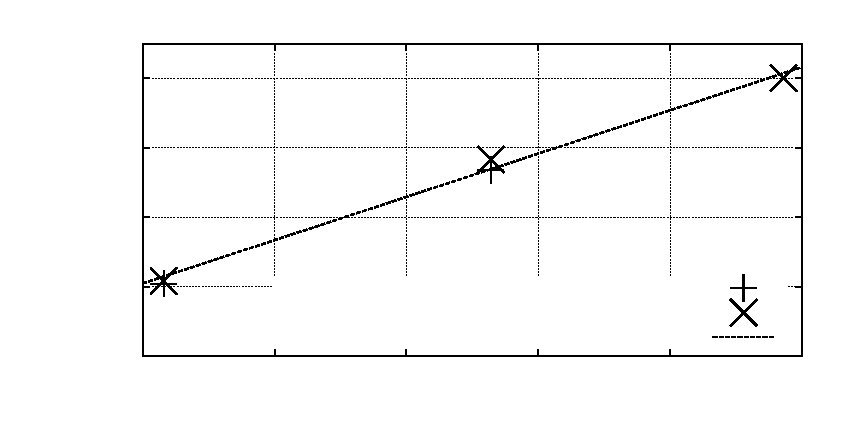
\includegraphics{div}}%
    \gplfronttext
  \end{picture}%
\endgroup

\caption{Průměr svazku v různých vzdálenostech od výstupu laseru}
\label{g:div}
\end{graph}


%STUPEŇ POLARIZACE
\begin{tabulka}[htbp]
\centering
\begin{tabular}{c|cccc}
maximální & 610 &  630 & 680 & 680 \\
minimální & 6 & 6 & 6 & 6 \\
\end{tabular}
\caption{Maximální a minimální naměřená relativní intenzita při různých orientacích polarizátoru}
\label{t:pol}
\end{tabulka}